\section{Methodology}
\label{sec:methodology}
In this section, we discuss the construction of the distributed sketch, sketchlet data structure, dynamic scaling, and query support in \textsc{Synopsis}. In most of those subsections, we present microbenchmarks which were run using a single machine (HP DL160 server with Xeon E5620 processor and 12 GB RAM) demonstrating the efficacy of individual aspects of the system. Our input data was sourced from NOAA North American Mesoscale (NAM) Forecast System \cite{noaa_nam}.

\subsection{Sketch}
\begin{figure*}
    \centerline{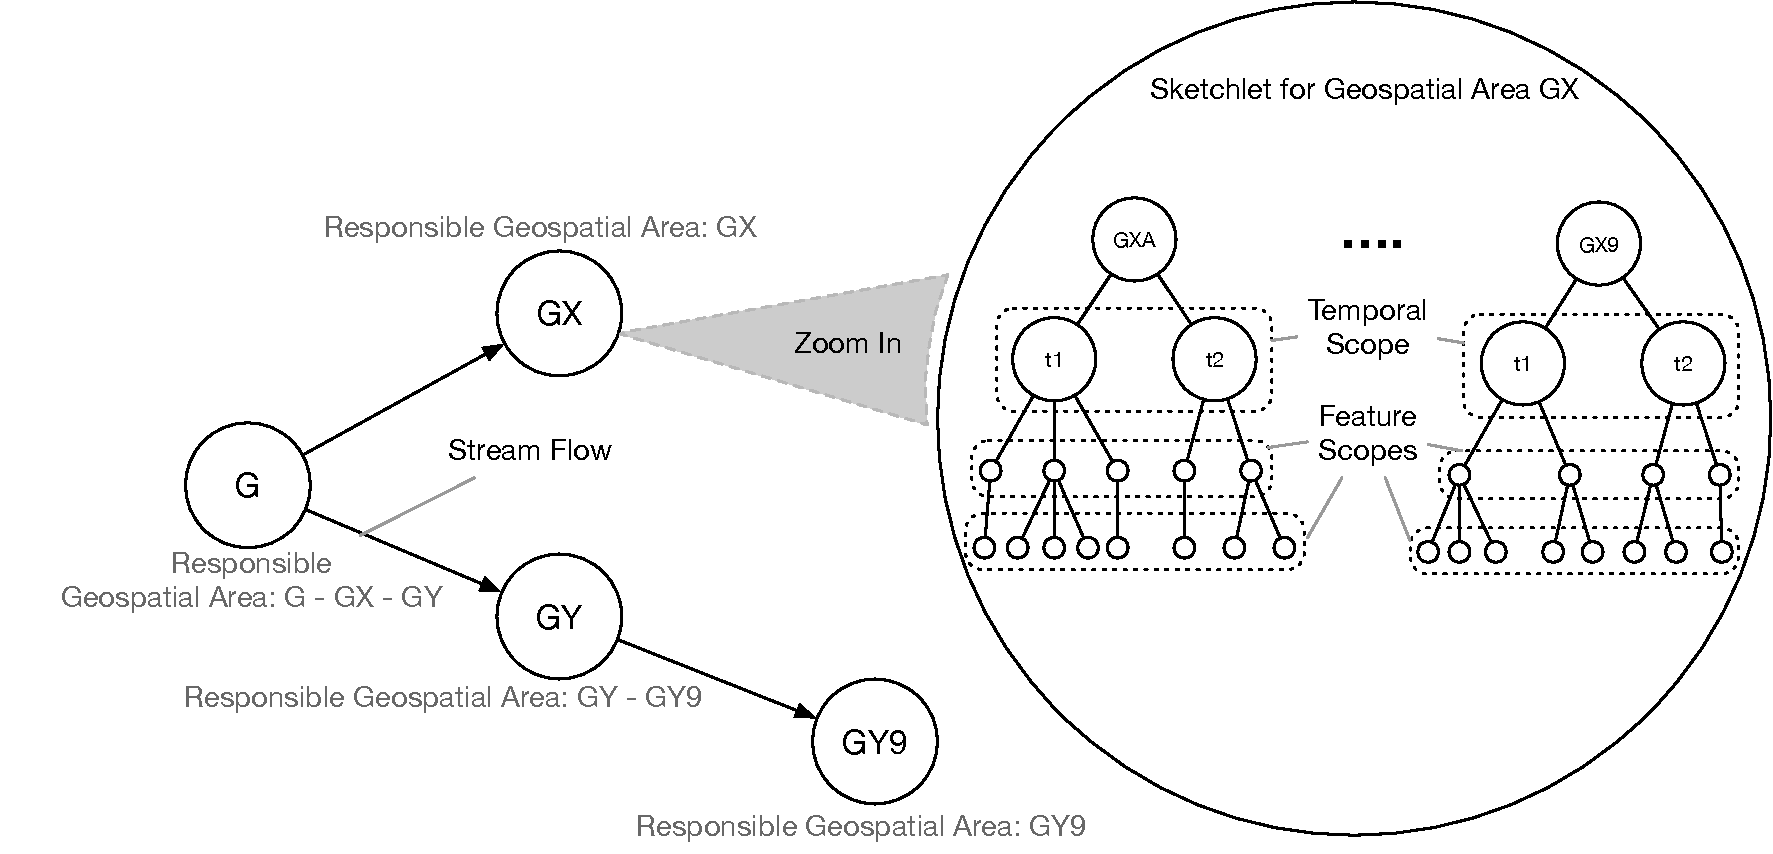
\includegraphics[width=0.8\textwidth]{figures/dist-sketch.pdf}}
    \caption{Demonstration of the distributed sketch for geospatiol region with the geohash prefix G. The sketchlets for geohash prefixes GX and GY have scaled out due to high volume of observations. A single sketchlet comprises of the SIFT data structure which is a forest of trees where each tree is responsible for a more specific geospatiol region.}
    \label{fig:dist-sketch}
\end{figure*}

The macroscopic view of the distributed sketch is one that comprises multiple sketchlets; each sketchlet executes on a different machine and is responsible for organizing data for a particular geospatial scope. The sketch is organized as a modified, distributed prefix tree. All the descendant nodes – the sketchlets – share a common prefix associated with the parent. Unlike traditional prefix trees, where the root node is an empty string, the root node is the coarsest granularity of the geohash i.e. the prefix that is common across all observations. Within a sketchlet all observations share the prefix associated with that sketchlet.

The sketch must be performant and flexible while being amenable to scaling operations. The sketch initiates scale-out operations to relieve memory pressure and preserve performance in the face of voluminous data. Scale-in operations are initiated by the sketch to conserve memory. Any sketchlet may serve as the conduit for incoming queries or analytic operations over the sketched spatiotemporal data: the sketch must be organized such that the sketchlets are not involved in redundant query evaluations or analytic operations. 

The geohash algorithm is well suited to our problem and plays a central role in the organization of the distributed sketch. Since the geohash algorithm represents a bounding box, it faciliates collation of observations from a particular geographical scope. This in turn allows us to redirect queries effectively and ensure data locality during query evaluations. Increases in the length of the geohash string correspond to geographically smaller bounding boxes being identified with increasing precision. This is also well-aligned with dynamic scaling maneuvers performed by the sketch to manage memory requirements and the availability of observational data. Scaling operations within the sketch are targeted. Scale-out operations target geospatial locations with increased density of observations to relieve memory pressure and alleviate performance bottlenecks. Scale-in operations target geolocations where there is a sparsity in available data to conserve memory.

Each sketchlet is responsible for real-time organization, summarization, and compaction of observational data from the geographical scope represented by the sketchlet’s geohash.  The sketchlet performs two operations. First, it extracts metadata from incoming observations. Metadata extracted from individual observations include: geolocations, chronological information, and features encapsulated within the observation.

Second, the sketchlet is responsible for effective summarization and compaction of measurements and accompanying spatiotemporal information extracted in the previous step. The sketchlet organizes its summarization of the observational data, as a forest of trees in a data structure called SIFT (Summarization Involving a Forest of Trees). The underlying principle within this data structure is \textbf{grouping} to exploit similarities in values reported within observations. This organization principle extends to all dimensions associated with the observations: spatial, temporal, and encapsulated features. The grouping principle allows us to preserve fidelity of the observational space while conserving memory footprints.

Each tree within the SIFT is rooted at a higher precision geohash than that associated with the sketchlet. For example, at a sketchlet with a geohash prefix, gx, the trees within the SIFT at that sketchlet are rooted at higher precision geohashes such as gxb, gxc, gxd, etc. An advantage of this approach is that the sketchlet partitions data from different regions within the larger geospatial scope into smaller regions. This partitioning allows the data structure to further exploit similarity in the observation values reported for that spatial scope. 

Within each SIFT tree, the second level is used to group observations based on their temporal properties. This approach allows us to exploit similarity in readings reported for a particular time-range. Note that as you traverse one of the trees within the forest, this organization means that all descendants of a temporal node correspond to measurements reported for a particular region for a particular temporal scope. The SIFT data structure also allows supporting finer-grained temporal resolutions for the recent past –- e.g., minutes, hours, day, weeks, etc. – and then target compaction operations that fold finer-grained temporal scopes into a coarser grained temporal scope as time advances. Specifically, our organizational structure that allows us to support varying levels of expressiveness for different temporal scopes – recent observations are represented more expressively. For example, on 3/2/2017 we may maintain subtrees at the minute level for 3:01 pm, 3:02 pm, etc., at 3/2/2017 @ 5:00 pm these subtrees will be folded into observations for the hourly temporal scope for 3:00-4:00 pm, and at 4:00 pm the next day (3/3/2017) these would then be folded into the coarser gained temporal bin for the previous day. 

The grouping concept also extends to individual features. Each feature occupies a level within an individual tree in SIFT. At each level, the range of values that a feature can take is broken up into a set of bins (corresponding to the range of values) that they take. These ranges are determined using a KDE function to ensure that the binning of features is representative of the observed density in the distribution of values for that feature at the particular spatiotemporal scope. Each node (or bin) maintains 5 variables min, max, standard deviation, mean, and the total number of observations to capture the values observed over that bin.  This is useful during the creation of synthetic datasets that are representative of the observational space for a particular spatiotemporal scope. A simplified version of the distributed sketch only for geospatial region with prefix G is depicted in Figure~\ref{fig:dist-sketch}. 

Our methodology of grouping and organizing the summarization information as a forest of trees accomplishes two key objectives. First, it captures the distribution of feature values across a spatiotemporal scope. Second, it supports targeted reductions in the observational data volumes while being representative of the observed feature values. This is in contrast to a random sampling scheme, which may be unable to recreate distributions with high fidelity for arbitrary spatiotemporal scopes or may drop significant values.

The organization of the sketchlet is such that it is amenable to scale-out and scale-in operations of the distributed sketch. Perhaps the most important feature provided by the SIFT data structure is support for scaling operations. For example, if a subregion – represented by a tree within the forest maintained at each sketchlet – has a higher density (and variability) of the reported observational values, that tree would have a correspondingly disproportionate memory footprint within the data structure. This allows us to target scaling maneuvers to particular sub-regions managed at a sketchlet to alleviate memory pressure.  During scale-in operations, descendants can be folded into the parent – the descendant’s SIFT is simply added as a tree to the SIFT maintained at the parent.

\subsection{Data Model}
Here we discuss the data model for observational data managed by Synopsis. Individual observations are geotagged and have chronological timestamps indicating where and when the observations were made. Location information is encoded as a $\langle latitude, longitude \rangle$ tuple. Observations are multidimensional with multiple features (e.g, temperature, humidity, wind speed, etc.) being reported in each observation. These features may be encoded as $\langle feature\_name, value \rangle$ tuples or may have predefined positions with the observational data's serialized representation. 

%TODO: does this add anything to the discussion? It seemed a bit out of place to me and you could say the same thing about other summary statistics maintained by the system (that they are not already encoded in the data) [malensek].
%Features encapsulated within these observations may be correlated.  Pairwise correlation coefficients are not encoded within the observations, but must instead be computed from the data. Observations are reported independently of each other, but for a given feature, values reported in successive observations may be correlated; once again, autocorrelation across successive measurements are not encoded in the observations. 

\textbf{SIFT:} The SIFT data structure is organized as a forest of trees. Data encapsulated within the observations are used to populate trees within SIFT. Each tree within SIFT has the geocoding information as its root node, temporal information at the second level, and individual features encapsulated within the observations at successive levels. The system may shuffle positioning of the features to conserve memory or speed up evaluations for dominant queries.

Additional nodes may be introduced to the trees within a SIFT to collate observations that fall within a certain range. In the case of chronological information these nodes correspond to different temporal scopes such as hours, days, weeks, months, and years. In the case of individual features, these nodes represent a binning of the feature values that correspond to the density in the distribution of observed feature values. Each feature node stores auxiliary information such as min, mean, max, standard deviation, and number of observations to capture statistical aspects about the distribution of values within the bin. Summary statistics are updated in an online fashion and keep pace with data arrival rates.

\textbf{Systems View of the Sketch:} The Synopsis sketch, comprising sketchlets dispersed over multiple machines, is a compact and memory-resident surrogate for the entire observational space. The sketch may be used for any purpose that regular, on-disk data is used for including but not limited to: query evaluations, assessing statistical properties of the data, and launching custom computations using well-known analytical engines. The system imposes no restrictions on the programming language or the type of processing logic that may be encoded within the computations. 

The Synopsis sketch is adaptive and evolves over time. The number of sketchlets comprising the sketch varies as the sketch performs scaling maneuvers to cope with data volumes and memory management. The number of trees within the SIFT  also varies over time as temporal scopes are aggregated, features binned, and sketchlets are spawned and fused during scaling operations.


\subsection{Sketchlet}
\label{sec:sketch}
The distributed sketch maintained by \textsc{Synopsis} is composed of many \emph{sketchlets} dispersed over a cluster of machines. Sketchlets maintain compact, multidimensional, tree-based representations of incoming data streams in the SIFT data structure. Each in-memory SIFT can be queried to retrieve statistical properties about the underlying data or discover how features interact. Due to the voluminous nature of these data streams, storing each individual record in main memory is not practical. Therefore, the queries supported by our framework are facilitated by compact, online metadata collection and quantization methods. These techniques ensure high accuracy while also conforming to the memory requirements of the system. To further improve accuracy, we bias our algorithms toward the most recent data points while reducing the resolution of the oldest.

\subsubsection{SIFT Structure}
\label{sec:sift}
SIFT instances are maintained as hierarchical trees with feature values stored in the vertices. Each level of the hierarchy, called a \emph{plane}, represents a particular \emph{feature type}, and traversing through vertices in this feature hierarchy reduces the search space of a query. Upon insertion of a multidimensional observation, each feature is arranged to form a \emph{path} through the tree and added based on the current feature hierarchy. Paths taken through the tree during a lookup are influenced by the specificity of the query, with additional feature expressions constraining the \emph{query scope}; an empty query would result in a scope that spans the entire tree. Figure~\ref{fig:sketch} demonstrates the structure of a tree within a SIFT and highlights a query and its scope. Note that any subset of the tree can be retrieved and manipulated in the same manner.

\begin{figure}[b!]
    \centerline{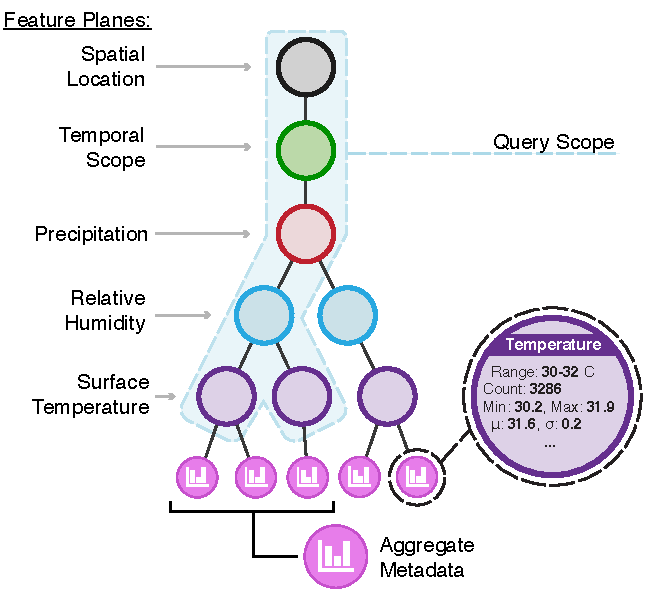
\includegraphics[width=3.2in]{figures/sketch.pdf}}
    \caption{A simplified SIFT tree with five feature planes and a sample query scope, leading to several metadata leaves. In production settings, these trees contain hundreds of thousands of vertices and edges.}
    \label{fig:sketch}
\end{figure}

Metadata records for paths through the feature hierarchy are stored at leaf nodes. Each record contains statistics that are updated in an online fashion using Welford's~method~\cite{welford1962note}. Welford's method maintains the number of observations, $n$, the running mean, $\bar{x}$, and the sum of squares of differences from the current mean, $S_n$, as in the following recurrence relation:
\begin{align*}
    \bar{x}_0 &= 0, S_0 = 0 \\
    \bar{x}_n &= \bar{x}_{n - 1} + \frac{x_n - \bar{x}_{n - 1}}{n} \\
    S_n       &= S_{n - 1} + (x_n - \bar{x}_{n - 1})(x_n - \bar{x}_n)
\end{align*}
Besides the observation count and running mean, this enables calculation of the variance and standard deviation of the observed values:
\begin{align*}
    \sigma^2 = \frac{S_n}{n} \hspace{2em} \sigma = \sqrt{\frac{S_n}{n}}
\end{align*}
Our implementation of Welford's method also includes cross-feature relationships, such as the correlation between temperature values and humidity or the reflectivity of the earth and cloud cover. This is achieved by maintaining the sum of cross products between features. Leaf nodes may be \emph{merged} to combine their respective summary statistics into a single aggregate summary. This allows queries to be evaluated across multiple sketchlets and then fused into a single, coherent result.

\subsubsection{Structural Compaction}
The number of unique feature types stored in the SIFT directly influences the size of the hierarchy, impacting memory consumption. However, the number of vertices and edges that must be maintained by each tree can be managed by manipulating the hierarchical configuration. For instance, the memory impact of features that exhibit high variance over a large range can be mitigated by placing them toward the top of the hierarchy, while boolean features or those with low variance should be situated toward the bottom of the tree. Consequently, we \emph{compact} the logical representation of the SIFT by aggregating vertices from the entire forest and reorienting the feature planes to conserve memory. One notable result of this process is that leaf vertices may be responsible for storing spatial locations of the data points rather than the root of the tree as depicted in our conceptual model of the SIFT; consider a dataset with sensor readings dispersed over fine-grained spatial areas. To allow efficient scaling in and out during tree migration to other sketchlets, full-resolution geohashes are stored in the hierarchy. If these full-resolution hashes are maintained near the root of the tree, each spatial region will effectively be allocated its own unique portion of the SIFT. 

Feature planes are reconfigured dynamically to achieve structural compaction based on their corresponding vertex \emph{fan-out} during the initial population of the trees. Boolean values or unique data points, such as a spatial location where a sensor resides, are moved toward the bottom of the tree. Using the observed ranges for each feature, a \emph{fan-out score} is calculated to determine the worst case impact of feature fan-out. Features with fan-out scores nearest to the overall mean score are pushed to the top of the hierarchy. This helps keep the trees as compact as possible near the root, with most expansion occurring near the leaves, leading to increased path similarity.  During this phase, full-resolution feature values are stored at each vertex, but once a steady state is reached the \emph{quantization} process begins to determine bin sizes and compact the feature planes further.

\subsubsection{Density-Driven Quantization}
Maintaining data points, statistics, and cross-feature relationships in memory at full resolution is infeasible when faced with voluminous datasets, even when load is balanced over several computing resources. To reduce the memory consumption of SIFT instances we perform \emph{quantization} --- targeted reduction of resolution --- which allows vertices in the tree to be merged, thus enabling single vertices to represent a collection of values. We determine which vertices should be merged by splitting each range of feature values into a configurable number of \emph{bins}. After quantization, each vertex represents a range of observations.

To determine the size and quantity of these bins, trees within the SIFT maintain additional metadata provided by the multivariate online kernel density estimation (oKDE) algorithm developed by Kristan et al. \cite{kristan2011multivariate}. While it is possible to recompute kernel density estimates periodically for each feature type using in-memory samples \cite{malensek2013autonomously}, the online approach afforded by oKDE requires less overall CPU usage and memory, which is crucial in streaming environments.  oKDE assimilates data incrementally at runtime to create a dynamic probability density function (PDF) for each feature type. The smoothing parameter used to create the PDF, called the \emph{bandwidth}, is selected autonomously using Silverman's rule \cite{silverman1986density}. Silverman's rule assumes that data tends to follow a normal distribution, which is generally true for naturally-occurring observations. However, we also allow the smoothing parameter be selectively reconfigured for different problem types. During the quantization process, these PDFs are used to ensure that each bin is assigned an approximately equal proportion of the feature density, while the overall number of bins is influenced by memory availability. As a result, the majority of values for a given feature type will be stored in small, highly-accurate bins.

Figure~\ref{fig:quantization} illustrates the quantization process for the \emph{surface temperature} feature in our atmospheric test dataset \cite{noaa_nam}: the highest densities of values are stored in the smallest bins (indicated by vertical lines under the curve), improving overall accuracy. To evaluate accuracy, we compare the mean values of each bin with the actual, full-resolution data points. Consequently, the \emph{standard error} ($\sigma_{\bar{x}}$) can be calculated from our running summary statistics to judge the accuracy level of the bins based on how well they are represented by the mean:
\begin{align*}
    \sigma_{\bar{x}} = \sqrt{\frac{S_n}{n^2}}
\end{align*}
This information is provided alongside any query results returned by the system. During initialization, we calculate the normalized error for each data point empirically (shown in the lower portion of Figure~\ref{fig:quantization}). For values that are observed less frequently, the error rate is higher; temperatures from 240 -- 260 Kelvin (-33.15 to -13.15 \degree C) reach a normalized root-mean-square error (NRMSE) of about 7\%. However, approximately 80\% of the values in the tree will be assigned to vertices with an error of about 0.5\%. In practice, this means that commonly-observed values returned by \textsc{Synopsis} will be within 0.25 Kelvin of their actual value.
%
\begin{figure}
    \centerline{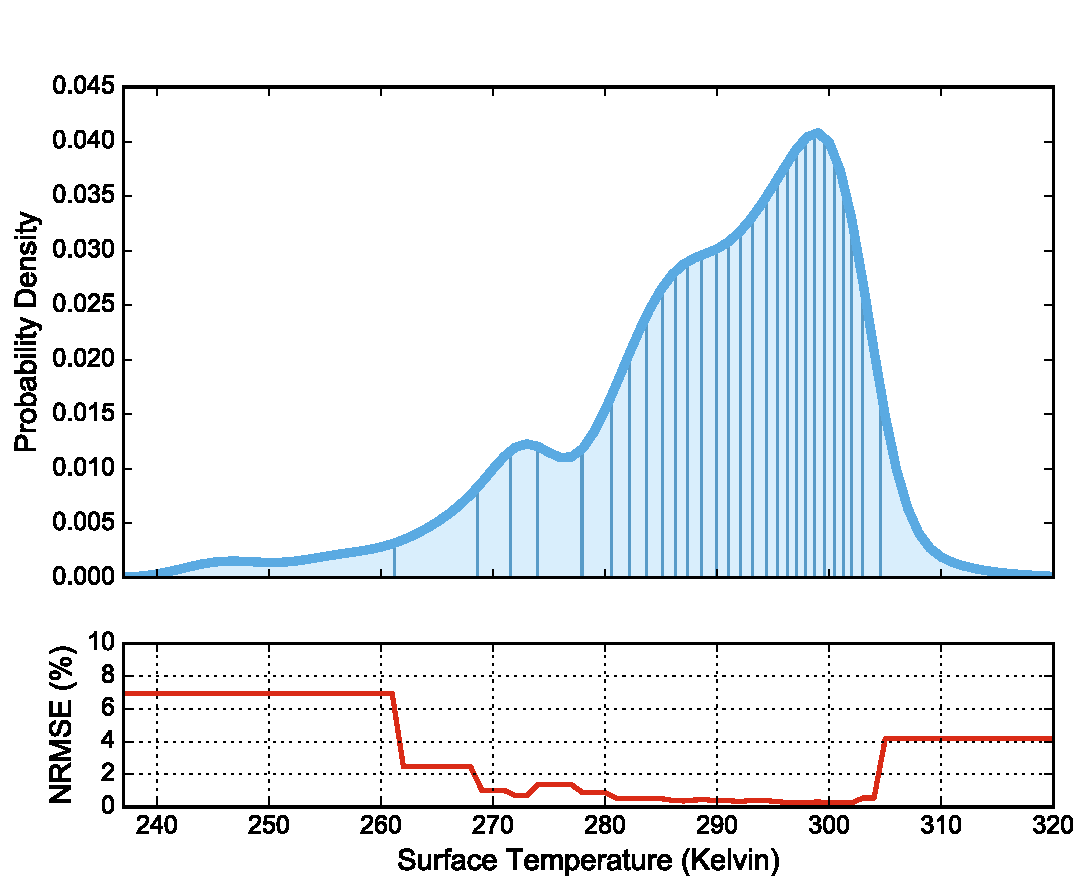
\includegraphics[width=3.5in]{figures/quantization.pdf}}
    \caption{A demonstration of the quantization process, with 29 vertex bins generated across the distribution of surface temperature values in our dataset. Each bin is indicated by a vertical line under the curve.}
    \label{fig:quantization}
\end{figure}
%
Table~\ref{tbl:tree-stats} compares full-resolution and quantized trees that were generated from a month of data with 20 unique features from our test dataset, which includes atmospheric information such as temperature, humidity, precipitation, and cloud cover. In this configuration, our autonomous quantization algorithm reduced memory consumption by about 62.4\%, which allows much more historical data to be maintained in each SIFT. Decreasing the memory footprint of the SIFT also allows larger geographical areas to be maintained by a single sketchlet.
%
\begin{table}[h!]
    \renewcommand{\arraystretch}{1.2}
    \caption{Tree statistics before and after our dynamic quantization algorithm over one month of ingested data.\vspace{-1em}}
    \label{tbl:tree-stats}
    \begin{center}
        \begin{tabular}{|l|c|c|c|}
            \hline
            \textbf{Metric} & \textbf{Original} & \textbf{Quantized} & \textbf{Change} \\
            \hline
            Vertices & 3,104,874 & 1,238,424 & -60.1\% \\
            \hline
            Edges    & 3,367,665 & 1,441,639 & -57.2\% \\
            \hline
            Leaves   & 262,792   & 203,216   & -22.7\% \\
            \hline
            Memory   & 1,710.6 MB & 643.1 MB  & -62.4\% \\
            \hline
        \end{tabular}
    \end{center}
\end{table}

\subsubsection{Temporal Dimensionality Reduction}
While our quantization approach enables \textsc{Synopsis} to retain large volumes of data in main memory, we also offer a temporal \emph{accuracy gradient} to ensure the most relevant data points are prioritized for high accuracy. This is achieved by iteratively removing tree paths from the SIFT hierarchy in the oldest subtrees, eventually phasing out old records. A user-defined ``length of study'' (for instance, 12 months) informs the system when dimensionality reduction can begin. As data ages, this process results in the creation of temporal accuracy bands.

Selective temporal dimensionality reduction proceeds in a bottom-up fashion, starting from the leaf nodes. Given a set of relevant vertices, neighboring bins are merged uniformly across the feature space. As the bins are merged, their respective metadata is also merged, reducing memory consumption. Given two metadata instances, merging results in half the memory footprint. However, it is worth noting that this process is irreversible; once metadata has been merged, it cannot be split at a later point in time. As time passes, entire portions of the feature hyperplane are compacted until a single metadata record is left for a particular temporal range. This allows users to still query the summary statistics and models for historical data, but at a lower level of accuracy.


%\subsection{Stream Partitioning}
%
\begin{figure}[h!]
    \centerline{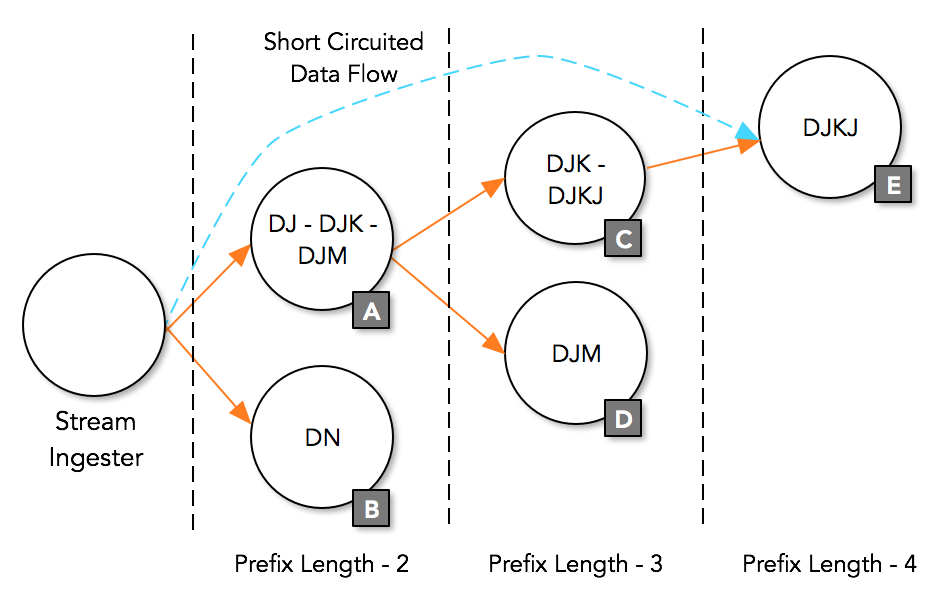
\includegraphics[width=3.5in]{figures/stream-partitioning.png}}
    \caption{An example of our stream partitioning approach based on the Geohash values of incoming packets.}
    \label{fig:stream-partitioning}
\end{figure}
%
Figure~\ref{fig:stream-partitioning} depicts a possible arrangement of the distributed sketch and the associated stream partitioning scheme corresponding to our example region.
The distributed sketch is arranged in a tree-like structure.
Stream ingesters act as root nodes of the tree and partition the stream among \textsc{Synopsis} nodes using a Geohash-based partitioning function.
Nodes closer to the root hold sketches corresponding to shorter Geohash strings, and therefore larger geographical regions.
For instance, nodes A and B in Figure~\ref{fig:stream-partitioning} are responsible for regions represented by Geohashes \emph{DJ} and and \emph{DN} respectively.
Node E, which is three edges deep from the stream ingester, is responsible for a smaller region, \emph{DJKJ}.

\textsc{Synopsis} is designed to ensure that regions corresponding to larger portions of the input streams (hence, more frequent updates) are moved to dedicated or less crowded nodes.
If a node decides to scale out a portion of the region it is currently responsible for, then the corresponding state (sketchlet and related metadata) is transferred over to the new computation and it starts to treat the stream packets corresponding to the scaled out region as pass-through traffic (Scaling out is explained in section~\ref{subsec:scaling-out}).
More specifically, the node will not process the stream packet, but instead updates its statistics based on the headers of the packet and forwards it to the destination child node. 
For instance, node A in Figure~\ref{fig:stream-partitioning} has scaled out two regions (\emph{DJK} and \emph{DJM}) to nodes C and D.
After these two scaling out operations, node A is responsible for all sub-regions in \emph{DJ} except for \emph{DJK} and \emph{DJM}.
Similarly, the sketch for the region \emph{DJKJ} is moved out of node C into node E as a result of subsequent scale-out operation.
It should be noted that the depth and span of the distributed sketch are dynamic and are constantly evolving according to the workload and operating conditions.

As the tree grows, having parent nodes pass traffic through to their children becomes inefficient because of higher bandwidth consumption as well as increased latency due to additional network hops the packets have to travel through.
To circumvent this, we allow \emph{short circuiting}, which directs traffic from stream ingesters straight to child nodes.
This is depicted in Figure~\ref{fig:stream-partitioning}, where the stream ingester directly sends data to node E instead of sending it through nodes A and C.
We use our gossiping subsystem to update parent nodes on child state information, which is useful for scaling in as explained in Section~\ref{subsec:scaling-in}.

\subsection{Coping with High Loads: Scaling out}
\label{subsec:scaling-out}
%
\begin{figure}[h!]
    \centering
    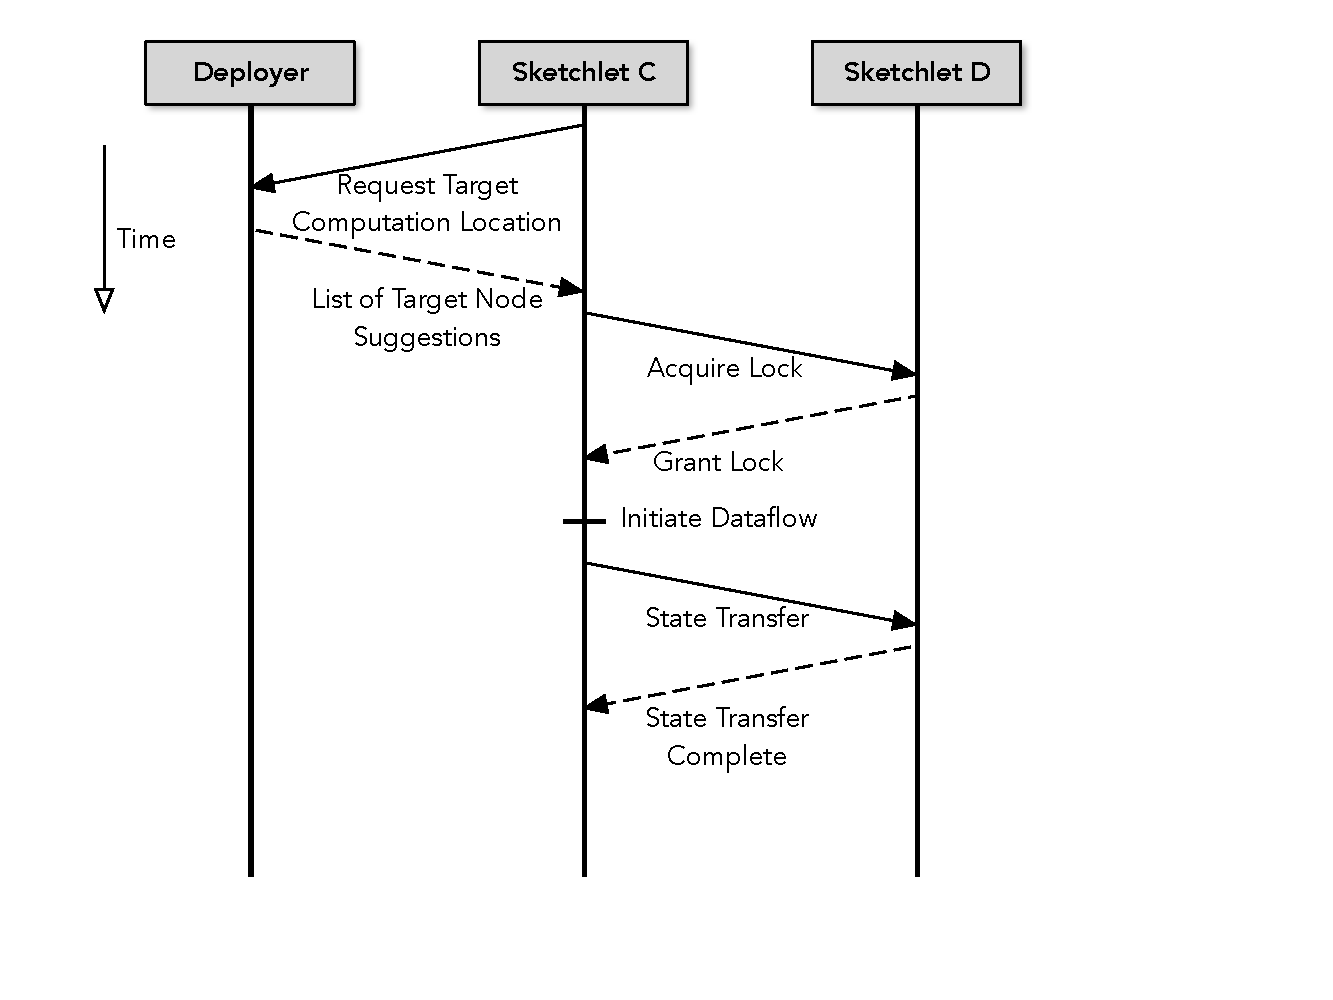
\includegraphics[scale=0.4, valign=t]{figures/scale-out.pdf}
    \caption{Scale-out protocol}
    \label{fig:scale-out-protocol}    
\end{figure}
There are two primary approaches to scaling a sketchlet that is experiencing high load: \emph{replication} and \emph{load migration}. In replication-based scaling, new sketchlets are spawned during high data arrival rates that are responsible for identical spatial scopes as their originating sketchlet. Assimilation of the newly-created sketchlet involves partitioning inbound streams directed to the original sketchlet. The upstream node (e.g.: stream ingester) is responsible for this partitioning, which may be performed in a skewed fashion with the new sketchlet receiving a larger portion of the inbound stream. Alternatively, inbound streams to the original sketchlet may also be partitioned in a round-robin fashion between the original and the newly-created sketchlet.
Using a replication-based scaling with a round-robin style stream partitioning is memory inefficient because of the possibility of multiple SIFT trees with significantly overlapping sets of vertices and edges.

In targeted load migration, particular geospatial scopes, i.e. SIFT trees are evicted from the original sketchlet to the newly created sketchlet during heavy load. Deciding which SIFT trees to migrate is based on data arrival rates and the rates at which particular SIFT trees are being updated.

%[malensek] NOTE: I removed this because it contradicts our discussion on the ability of the sketch to merge arbitrary states (even duplicated state -- in fact, that makes things easier). I think there are plenty of other reasons why replication-based scaling is weaker anyway.
%Replication-based scaling introduces a challenge during query evaluations in that the query must be forwarded to all nodes responsible for a particular scope and the results merged; depending on the nature of these queries (for e.g., correlation analysis and inferential queries) merging of results may be difficult to accomplish without extensive state synchronizations.
%TODO: lines about how scaling in can be difficult in replication setting
In \textsc{Synopsis}, we use targeted load migration for scaling out.
Our implementation closely follows the MAPE loop~\cite{maurer2011revealing} which comprises four phases: monitor (M), analyze (A), planning (P) and execution (E).
%The monitoring task as shown in Figure~\ref{fig:process-monitor} periodically probes every \textsc{Synopsis} task to gather two performance metrics as part of monitoring phase.
A \textbf{monitoring} task within every sketchlet periodically gathers two performance metrics:
\begin{enumerate}[leftmargin=*]
	\item \textbf{Length of the backlog:} This represents the number of unprocessed messages in the queue. If the sketchlet cannot keep up with the incoming data rate, then the backlog will grow over time.
	\item \textbf{Memory pressure:} Each sketchlet is allocated a fixed amount of memory. 
	Exceeding these memory limits creates memory pressure causing extended garbage collection cycles and increased paging activity, eventually leading to reduced performance.
	The monitoring task continuously records the memory utilization and triggers scaling activities.
\end{enumerate} 

The objective of scaling out is to maintain the \emph{stability} at each sketchlet.
We define stability as the ability to keep up with incoming data rates while incurring a manageable memory pressure.  During the \textbf{analyze} phase, we use threshold-based rules \cite{lorido2012auto} to issue scale-out recommendations to sketchlets, which are issued if \textit{either} of the following rules are consistently satisfied for a certain number of monitoring cycles:
\begin{itemize}[leftmargin=*]  
\item Backlog growth, which indicates that a portion of the load needs to be migrated to a different cluster-node.
\item High overall memory utilization above a threshold, which is usually set below the memory limits to allow a capacity buffer for the process to avoid oscillation.
\end{itemize}
Upon receiving a scale out recommendation during monitoring, the sketchlet executes the \textbf{planning} and \textbf{execution} phases.

During the planning phase, the sketchlet chooses portion(s) of the region within its current purview, i.e. a set of SIFT trees, to be handed over to another sketchlet.
For this task, it relies on performance metrics it maintains for each subregion and a numeric value provided by the scale-out recommendation that measures how much load should be migrated.
These metrics includes the data rate and the memory consumption for each subregion.
If the backlog growth based threshold rule has triggered the scale out operation, the subregion metrics are sorted based on their update rates in the descending order. Otherwise they are sorted based on their memory consumption.
Then a simple bin-packing algorithm is used to choose a minimum set of subregions for migration such that the excess load is removed from the current sketchlet.

Only a single scaling operation takes place at a given time per sketchlet, which is enforced by a mutex lock.
Further, every scaling operation is followed by a \textit{stabilization period} where no scaling operation takes place and system does not enter the monitoring phase for the next MAPE cycle.
The objective of these constraints is to avoid oscillations in scaling activities; for instance, repetitively scaling out in the presence of memory pressure could result in overprovisioning, which would then lead to recurring scale-in operations.
%

Figure~\ref{fig:scale-out-protocol} depicts the phases of the scale-out protocol with respect to our example in Figure~\ref{fig:dist-sketch} when sketchlet C is scaling out to sketchlet D.
Once the sketchlet decides on subregions to scale, it initiates the scale-out protocol by contacting the \emph{deployer} process, which is responsible for launching tasks.
In this message, it includes a list of preferred target sketchlets for the load migration as well as memory requirements and expected message rate for the load.
The preferred sketchlet set includes the sketchlets that already hold other subregions.
It minimizes the number of sketchlets responsible for each geographical region to reduce communication during query evaluations.
% system stability
\begin{figure*}[h!]
    \begin{subfigure}{0.48\textwidth}
            \centering
            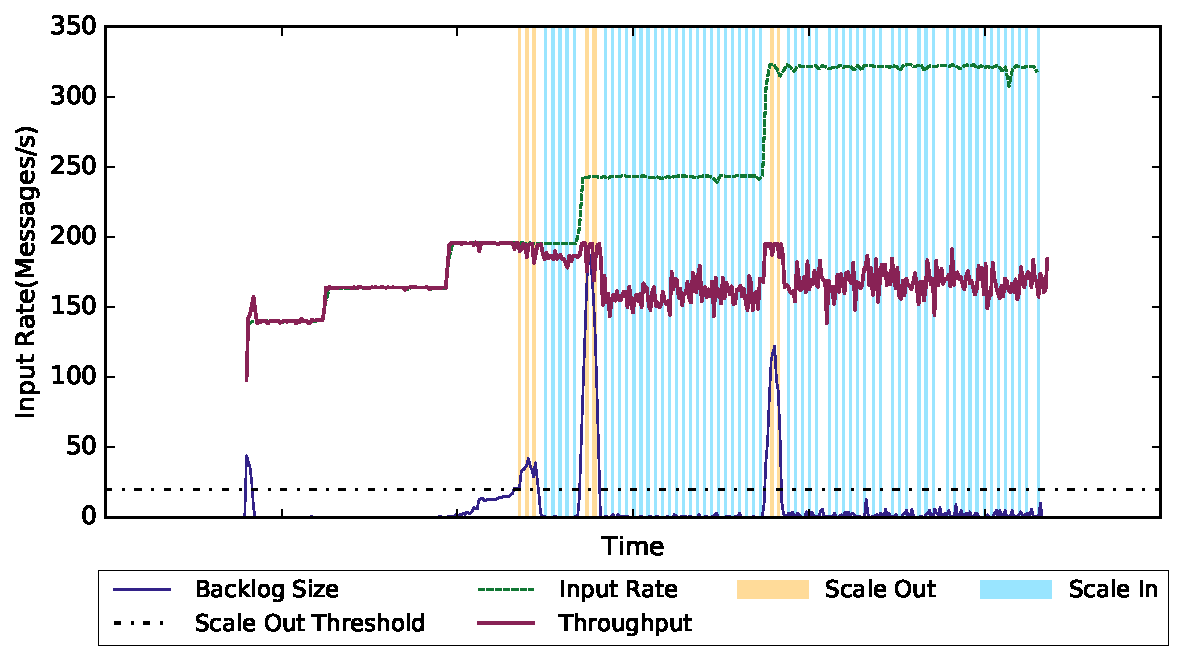
\includegraphics[scale=0.42]{figures/stability_partial.pdf}
            \caption{Triggered by backlog growth based threshold rules}
            \label{fig:stability-backlog}
    \end{subfigure}
    \begin{subfigure}{0.48\textwidth}
            \centering
            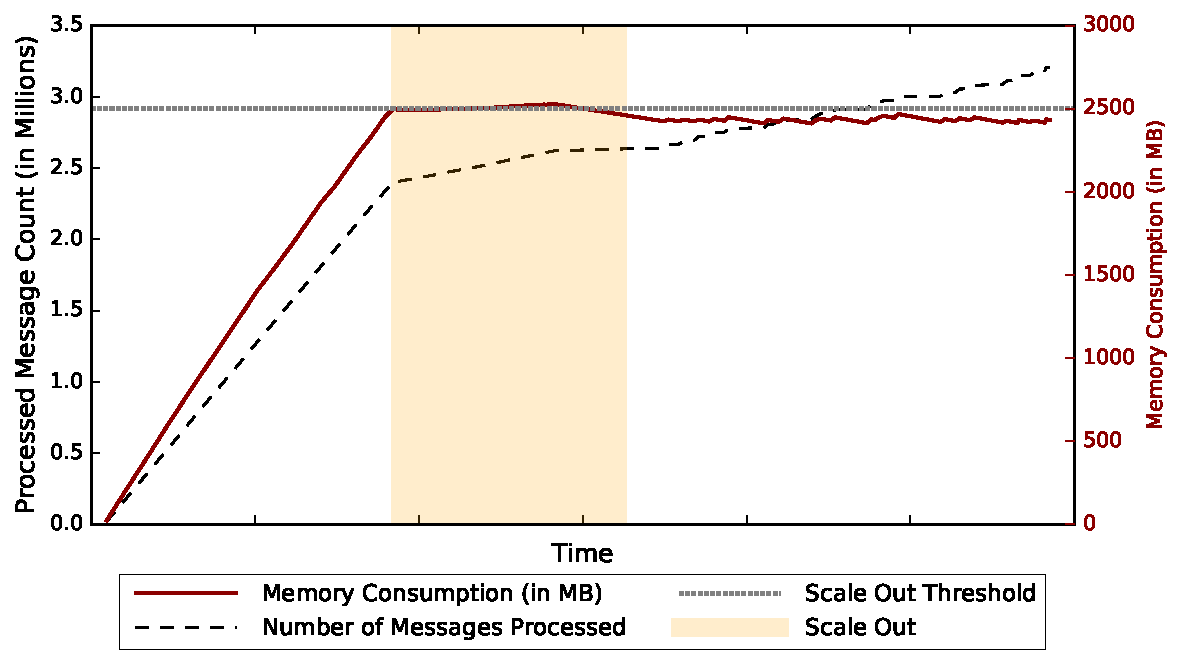
\includegraphics[scale=0.42]{figures//mem_stability.pdf} 
            \caption{Triggered by memory usage based threshold rules}
            \label{fig:stability-mem}
    \end{subfigure}
    \caption{Scaling out based on backlog growth and memory usage enables maintaining stability at an individual sketchlet}
    \label{fig:system-stability}
\end{figure*}
%
The \textsc{Synopsis} deployer component has an approximate view of the entire system constructed through gossip messages. This includes the memory pressure and cumulative backlog information for each sketchlet.
Based on this view and the information present in the request, the deployer replies back with a set of candidate target sketchlets.
Only if a suitable candidate cannot be found from the set of current sketchlets will a new sketchlet be spawned.
Upon receiving a response from the deployer, the sketchlet (parent) contacts the target sketchlet (child) and tries to acquire the mutex.
A lock will be granted only if the target can accommodate the load and no other scaling operations are taking place.
If the lock acquisition fails, another candidate from the list is attempted; otherwise, the parent sketchlet will create a pass-through channel and direct traffic corresponding to migrated regions towards the child sketchlet.
Once this process is complete, the parent sketchlet will initiate a state transfer asynchronously using a background channel to ensure the stream data flow is not affected, and update the child sketchlet's memory utilization metrics to account for the pending state transfer.

As the data flow tree grows with scaling out operations, having parent sketchlets pass traffic through to their children becomes inefficient because of higher bandwidth consumption as well as increased latency due to the additional network hops the packets have to traverse through.
To circumvent this, we allow \emph{short circuiting}, which redirects traffic from stream ingesters straight the downstream sketchlets.
For instance, stream ingesters will send data directly to sketchlet D using the short circuited route bypassing sketchlets A and C in Figure~\ref{fig:dist-sketch}. 
We use our gossiping subsystem to update parent sketchlets about the child's performance metrics required for scaling in (\S\ref{subsec:scaling-in}).

We evaluated how each of these rules triggers dynamic scaling activities to maintain the system stability.
For this experiment, we have enabled only a single threshold-based rule at a time to demonstrate its effectiveness.
To evaluate the backlog based threshold rule, we captured how backlog length and throughput at an individual sketchlet varies with the input rate.
The sketchlet immediately received data from stream ingesters, hence the input rate observed at the sketchlet closely resembled the varying data ingestion rate.
As shown in Figure~\ref{fig:stability-backlog}, scaling out helps a sketchlet to keep pace with the variations in the workload, which in turn, causes the backlog to stay within a safe range.
This microbenchmark also demonstrates infrequent, rapid scale-out and continuous, gradual scale-in as explained in \S\ref{subsec:scaling-out}.

Figure~\ref{fig:stability-mem} demonstrates how memory consumption based threshold-based rules trigger scaling maneuvers to maintain the stability of an individual sketchlet.
We have used a 0.45 of the total available memory for a JVM process as the upper threshold for triggering a scale-out operation.
In certain occasions, it is required to perform multiple consecutive scaling out operations (interleaved with the cooling down periods) to bring the memory usage to the desired level due to the increased memory utilization caused by the data ingestion happening in the background.

%Completing the scale-out protocol quickly is important because it can release mutual exclusive locks in both origin and target \textsc{Synopsis} nodes quickly and participate in other scaling activities soon after the stabilization period.
%
%
\begin{figure}[b!]
    \centering
    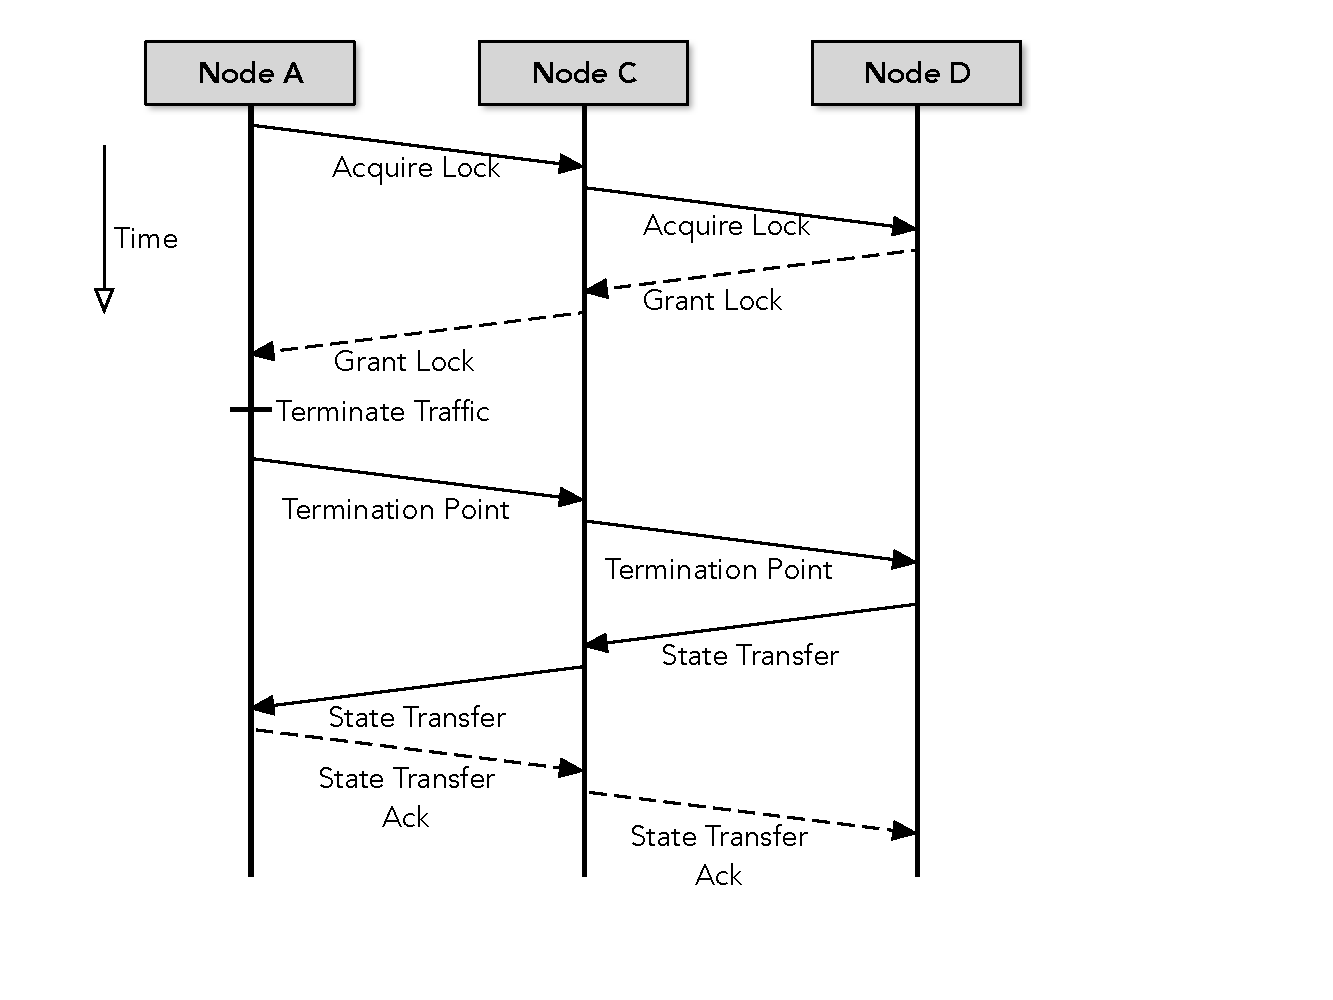
\includegraphics[scale=0.4, valign=t]{figures/scale-in.pdf} 
    \caption{Scale-in protocol}
    \label{fig:scale-in-protocol}
\end{figure}
\subsection{Scaling In: Conserving Resources}
\label{subsec:scaling-in}
During scaling in, sketchlets merge back some of the subregions scaled out previously.
This ensures better resource utilization in the system in addition to efficient query evaluations by having to contact fewer sketchlets.
Scaling in is also guarded by the same mutex lock used for scaling out (only one scale-out or scale-in operation takes place at a given time) and is also followed by a stabilization period.

Monitoring and analysis during scale-in operations proceeds similarly to scaling out, except for the obvious change to the threshold-based rules: now \textit{both} memory pressure and backlog length metrics should consistently record values below a predefined lower threshold.
When scaling in, we use a less aggressive scheme than scaling out; a single subregion is acquired during a single scale-in operation.
Scaling in is more complex than scaling out because it involves more than one sketchlet in most cases.
At this point, it is possible that further scale-out operations have taken place in the scaled out subregion after the initial scale-out.
For instance, if sketchlet A in Figure~\ref{fig:dist-sketch} decides to scale-in the subregion \emph{DN}, then it must communicate with sketchlets C and D.

The scale-in protocol starts with a lock acquisition protocol similar to the scaling out protocol, but involves locking the entire subtree.
The steps are depicted in Figure~\ref{fig:scale-in-protocol} with respect to our example in Figure~\ref{fig:dist-sketch} where sketchlet C is scaled in.
As per our example, sketchlet A will have to acquire locks for both sketchlets C and D.
Locks are acquired in a top-to-bottom fashion where parent locks itself and then attempts to lock the child.
If lock acquisition fails for any part of the subtree, the scale-in operation is aborted and the monitoring process starts the next iteration of the MAPE loop immediately.
If the lock acquisition is successful, then data flow to the child sketchlet corresponding to this subregion is immediately terminated.

The state acquisition phase begins next.
To ensure that \textsc{Synopsis} does not lose any messages, the initiating sketchlet sends a \emph{termination point} control message to the child sketchlet.
The termination point is the sequence number of the last message sent to the child sketchlet either by the parent itself or by the short circuit channel.
%It may be possible that the child has already processed this message and updated its sketch by the time it receives the termination point control message, but in extreme cases the termination point control message may get processed before the actual stream packet with the same sequence number.
%This is because control plane and data plane use separate channels and also due to the possibility of data plane messages are being queued before processing.
Once the child sketchlet has processed every message up to the termination point, it sends out termination point messages to all relevant child sketchlets. In our example, sketchlet C sends a termination point control message to D upon processing the stream packet corresponding to the termination point sent by sketchlet A.
After the entire subtree has seen all messages up to the termination point, they acknowledge the initiator sketchlet and start transferring their states asynchronously.
Once the parent sketchlet receives acknowledgments from the entire subtree, it starts propagating the protocol end messages to initiate lock releasing.
Locks are released from the bottom to top in the subtree, with the parent sketchlet releasing its lock after each child has released its lock.
%
\subsection{Query Evaluations}
\label{subsec:query-eval}
\textsc{Synopsis} incorporates support for user-defined queries that are evaluated over the distributed sketch.  Queries can be specified by the user in a SQL-like format or with JSON-based key-value descriptions similar to GraphQL~\cite{graphql}. Exact-match, range-based, and summarization queries are all supported over spatiotemporal bounds and individual feature values. The following example depicts how SQL-like queries can be formulated for evaluation over the sketch.

\begin{Verbatim}[fontsize=\footnotesize]
SELECT MEAN(precipitation), MAX(wind_speed)
WHERE temperature > 20 AND temperature < 30
AND humidity > .8 AND CORRELATION(
    cloud_cover, precipitation) < -0.25
\end{Verbatim}

Depending on scaling operations and the spatial scope of the queries, evaluations are carried out on one or more sketchlets. Information on the placement of sketchlets in the system and their corresponding feature scopes is maintained at each sketchlet in a geohash prefix tree, with changes propagated through the network in an eventually-consistent manner as data is ingested and scaling maneuvers occur.

The entry point for these queries, called the \emph{conduit}, may be any of the sketchlets comprising the distributed sketch. During query evaluations, the first step is to identify the set of sketchlets that are relevant to the query. The conduit consults its prefix tree to locate sketchlets based on spatial, chronological, and feature constraints specified by the user. After this process is complete, the conduit forwards the queries on to the sketchlets for evaluation and supplies the client with a list of sketchlets that will respond to the query. As queries execute, results are streamed back to the client and merged by the client API. This strategy ensures that I/O and processing activities are interleaved on the client side.

Our distributed prefix tree enables query evaluations during both scaling in and out. For instance, when a conduit attempts to forward a query to a child sketchlet that is undergoing a scale-in operation, the request will be redirected to the its parent sketchlet. This process can continue recursively up through the network, ensuring queries will reach their destination.

\subsubsection{Query Types}
Queries supported by \textsc{Synopsis} fall into six categories:
\begin{description}[leftmargin=*]
    \item[Relational Queries] describe the feature space in the context of the hierarchical trees within our SIFT data structure and may target ranges of values under certain conditions. For example, ``What is the relationship between temperature and humidity during July in Alaska, USA, when precipitation was greater than 1 centimeter?'' These queries return a subset of the overall sketch that includes any other matching feature values as well.
    % Subsketches may be manipulated and inspected on the client side, and then reused in subsequent queries to request more detail or broaden the query scope. Relational queries can optionally return statistical metadata stored in the leaf nodes of the tree; this is also supported by our statistical query functionality.

    \item[Statistical Queries] allow users to explore statistical properties of the observational space. For example, users can retrieve and contrast correlations between any two features at different geographic locations at the same time. Alternatively, queries may contrast correlations between different features at different time ranges at the same geographic location. These queries also support retrieval of the mean, standard deviation, and feature outliers based on Chebyshev's inequality \cite{knuth1968art}.

    \item[Density Queries] support analysis of the distribution of values associated with a feature over a particular spatiotemporal scope. These include kernel density estimations, estimating the probability of observing a particular value for an observation, and determining the deciles and quartiles for the observed feature.% Kernel density estimations can request the function itself, an integral over a range of values, or the probability of a single value.

    \item[Set Queries] target identification of whether a particular combination of feature values was observed, estimating the cardinality of the dataset, and identifying the frequencies of the observations. Each type of set query requires a particular data structure, with instances created across configurable time bounds (for instance, every day). Set membership is determined using space-efficient bloom~filters~\cite{bloom1970space}, while cardinality (number of distinct elements) queries are supported by the HyperLogLog~\cite{flajolet2007hyperloglog} algorithm.

%To determine set membership, we use Bloom filters may produce false positives, but never false negatives. Besides returning a \texttt{true} or \texttt{false} result to the user, membership queries also include the probability of the answer being a false positive.  Set HyperLogLog is able to estimate cardinality with high accuracy and low memory consumption. Finally, observation frequencies are provided by the count-min data structure \cite{cormode2005improved}. Count-min is structurally similar to a bloom filter, but can be used to estimate the frequency of values within a particular error band. Frequency queries are accompanied by their associated confidence intervals and relative error.

\item[Inferential Queries] enable spatiotemporal forecasts to be produced for a particular feature (or set of features). Discrete inferential queries leverage existing information in the distributed sketch to make predictions; aggregate metadata stored in the leaves of the tree can produce two-dimensional regression models that forecast new outcomes across each feature type when an independent variable of interest changes.

%In their continuous form, inferential queries are backed by machine learning models that are \emph{installed} for a particular time window and can be trained using either the sketch or new, full-resolution values as they arrive. Continuous inferential queries can stream predictions back to the client on a regular interval, or a subsequent query can reference a particular model and parameterize it to make a single prediction. Our current implementation of \textsc{Synopsis} supports multiple linear regression, but our machine learning interface allows new models to be plugged into the system at run time.

\item[Synthetic Data Queries] allow users to request the system to generate representative datasets based on the distributions stored in the sketch. Synthetic data is generated in an online fashion by sampling from the underlying distributions and then streamed to client applications for analytics. The size of the dataset may also be specified; for instance, 10\% of the volume of the original data points.
\end{description}
%
\begin{table}[h!]
    \renewcommand{\arraystretch}{1.2}
    \caption{Local sketchlet evaluation times for each query type (averaged over 1000 iterations). \vspace{-1em}}
    \label{tbl:query-times}
    \begin{center}
        \begin{tabular}{|l|c|c|}
            \hline
            \textbf{Query Type}      & \textbf{Mean (ms)} & \textbf{Std. Dev. (ms)} \\
            \hline
            Density                  & 0.007                    & 0.005 \\
            \hline
            Set Cardinality          & 0.154                    & 0.088 \\
            \hline
            Set Frequency            & 0.036                    & 0.019 \\
            \hline
            Set Membership           & 0.015                    & 0.009 \\
            \hline
            Statistical               & 0.002                    & 0.001 \\
            \hline
            \hline
            Tree Only (5 km)        & 46.357                   & 1.287 \\
            \hline
            Tree + Meta (5 km)      & 40.510                   & 6.937 \\
            \hline
            Tree + Meta (25 km)     & 47.619                   & 6.355 \\
            \hline
            Tree + Meta (800 km)    & 53.620                   & 6.818 \\
            \hline
        \end{tabular}
    \end{center}
\end{table}
Table~\ref{tbl:query-times} outlines local tree traversal times for query evaluations. These queries were separated into two groups: conventional lookups and tree retrievals. Conventional lookups include density queries, set queries, and statistical queries, while tree retrievals request targeted portions of the overall feature space as a tree.  Note that while conventional lookups do not return a tree structure to the client, they still require a tree traversal to resolve. In general, tree retrievals consume more processing time due to their serialization and I/O costs; however, it is worth noting that varying the geographical scope across sketchlet sizes from 5km to 800km did not result in a proportionate increase in processing time. Overall, the sketch provides low-latency query evaluations for each query type.

\subsection{Coping with Failures in Synopsis}
\textsc{Synopsis} relies on passive replication to recover from sketchlet failures because active replication increases resource consumption significantly and it is infeasible to use upstream backups because the state of a sketchlet depends on the entire set of messages it has processed previously \cite{castro2013integrating}.

Support for fault tolerance is implemented by augmenting the distributed sketch with a set of secondary sketchlets.
A sketchlet is assigned a set of $n$ secondary sketchlets on different machines to ensure \textsc{Synopsis} can withstand up to $n$ concurrent machine failures.
In our implementation, we used two secondary sketchlets ($n=2$) assigned to each sketchlet.
A primary sketchlet periodically sends the changes to its in-memory state as an \emph{edit stream} to its secondary sketchlets.
The secondary sketchlets, which act as the sink to the edit stream, serialize incoming messages to persistent storage.
This incremental checkpointing scheme consumes less bandwidth compared to a periodic checkpointing scheme that replicates the entire state \cite{castro2013integrating}.
By default, \textsc{Synopsis} uses the disk of the machine executing the secondary sketchlet as the persistent storage, but highly-available storage implementations such as HDFS~\cite{borthakur2008hdfs} can be used if necessary.
To reduce resource footprints, secondary sketchlets do not load the serialized state into memory unless they are promoted to being a primary.

System-wide incremental checkpoints are orchestrated by a special control message emitted by the stream ingesters.
\textsc{Synopsis} uses upstream backups at stream ingesters to keep a copy of the messages that entered the system since the last successful checkpoint.
In case of a failure, all messages since the last checkpoint will be replayed.
Sketchlets are implemented as idempotent data structures using message sequence numbers, hence they will process a replayed message only if it was not processed before.
The interval between incremental checkpoints can be configured based on time or the number of emitted messages.
Frequent checkpoints can incur high overhead, whereas longer periods between successive checkpoints consume more resources for upstream backups and require longer replay durations in case of a failure.

Membership management is implemented using Zookeeper~\cite{hunt2010zookeeper}, which is leveraged to detect failed sketchlets.
Upon receiving notification of a primary sketchlet failure, a secondary sketchlet assumes the role of primary through a leader election algorithm.
The secondary will start processing messages immediately and begins populating its state from persistent storage in the background.
Given this mode of operation, there may be a small window of time during which the correctness of queries are impacted.
This is rectified once the stored state is loaded to memory and the replay of the upstream backup is completed.
The SIFT's support for merge operations as well as its ability to correctly process out of order messages is useful during the failure recovery process.

As per our fault tolerance scheme, the \textit{total time to recover from the failure} ($T_{total}$) can be modeled as follows.
\begin{align*}
    T_{total} &= T_{d} + \max{(T_{l}, T_{r})}      
\end{align*}
where $T_{d}$ = \textit{time to detect a failure}, $T_{l}$ = \textit{time to load persisted state} and $T_{r}$ = \textit{replay time for messages at the upstream node}.

The time required to detect failures mainly depends on the session timeout value used by Zookeeper to detect lost members and the delay in propagating the notification to other members. With a $5s$ session timeout in an active cluster, we observed a mean notification propagation delay of $5.5s$ (std. dev. = $0.911s$, $95^{th}$ percentile = $6.000s$). Configuring a lower session timeout will increase the chance of false positives if sketchlets become non responsive for a while due to increased load or system activities such as garbage collection. The time required to load the persisted storage depends on the size of the serialized sketchlet; we benchmarked the time it takes to repopulate the state in all sketchlets after ingesting NOAA data for 2014. The mean state re-population time was recorded as $16.602s$ with std. dev. = $23.215s$ and $95^{th}$ \%ile = $70.877s$. Replay time mainly depends on the checkpointing interval as well as the message ingestion rate. With a checkpointing interval of 10000 messages, we experienced a mean value of $0.662s$ (std. dev. = $0.026s$, $95^{th}$ \%ile = $0.707s$) to replay an upstream buffer.


